\newpage
\section{Pregled i analiza naučnoistraživačkih radova}

U ovom poglavlju dat je pregled relevantnih naučnoistraživačkih radova iz oblasti vizuelne detekcije vatre i dima, s posebnim fokusom na pristupe primjenljive na skup podataka D-Fire \cite{dfire,kaggle}. Analiza obuhvata šest radova koje su pojedinačno obradili članovi tima, a cilj pregleda je sagledavanje postojećih metodologija, poređenje njihovih performansi i ograničenja te definisanje smjernica za izbor i razvoj modela u nastavku projekta.

Redoslijed potpoglavlja prati razvoj od općeg pregleda dubokog učenja i tradicionalnih metoda obrade slike, preko hibridnog pristupa zasnovanog na analizi boja i kontura, do savremenih jednofaznih detektora iz porodice YOLO (Tabela~\ref{tab:pregled}). Svaka analiza obuhvata sažetak rada, korištene metode, ostvarene rezultate, prednosti i nedostatke te povezanost s projektnim zadatkom.

\begin{table}[H]
\centering
\small
\begin{tabularx}{\linewidth}{@{}c>{\raggedright\arraybackslash}p{2.5cm}>{\raggedright\arraybackslash}p{3.7cm}>{\raggedright\arraybackslash}X>{\raggedright\arraybackslash}p{3.0cm}@{}}
\toprule
\textbf{Dio} & \textbf{Autor analize} & \textbf{Analizirani rad} & \textbf{Pristup} & \textbf{Skup podataka u radu}\\
\midrule
1 & \AutorA & Elhanashi i sar. (2025), \emph{Applied Sciences} \cite{elhanashi} & Sistematski pregled metoda dubokog učenja (80 studija) & Pregled oko 30 skupova, uključujući D-Fire\\
2 & \AutorB & Ahmad i Osman (2021), \emph{Sulaimani J.\ Eng.\ Sci.} \cite{ahmad} & Pregled tradicionalnih metoda obrade slike & Bez vlastitog eksperimenta\\
3 & \AutorC & Buriboev i sar. (2025), \emph{Sensors} \cite{buriboev} & Hibrid: analiza boja i kontura + CNN & D-Fire (21.527 slika)\\
4 & \AutorD & Ramos i sar. (2025), \emph{Results in Engineering} \cite{ramos} & Poređenje YOLOv8--YOLO11 & Roboflow Fire and Smoke (9.796 slika)\\
5 & \AutorE & Li i sar. (2025), \emph{IEEE Access} \cite{ligsf} & GSF-YOLOv8 (modifikacija YOLOv8) & D-Fire\\
6 & \AutorF & Li i sar. (2025), \emph{Front.\ Environ.\ Sci.} \cite{liyologx} & YOLOGX (modifikacija YOLOv8) & D-Fire\\
\bottomrule
\end{tabularx}
\caption{Pregled analiziranih naučnoistraživačkih radova.}
\label{tab:pregled}
\end{table}

\textbf{Napomena o poređenju rezultata.} Vrijednosti prikazane u nastavku preuzete su iz izvornih publikacija i nisu rezultat vlastitih eksperimenata tima. Direktno brojčano poređenje rezultata između različitih radova nije metodološki opravdano zbog razlika u korištenim skupovima podataka, omjerima podjele na skupove za treniranje i testiranje te definicijama evaluacijskih metrika.
% =====================================================================
%  DIO 1 -- Elhanashi i sar. (2025): pregled dubokog učenja
% =====================================================================
\clearpage
\subsection{\texorpdfstring{\AutorA}{Ime Prezime} --- Pregled dubokog učenja za ranu detekciju vatre i dima}

\paperbox{\AutorA}
  {A.\ Elhanashi, S.\ Essahraui, P.\ Dini i S.\ Saponara (Univerzitet u Pisi), „Early Fire and Smoke Detection Using Deep Learning: A Comprehensive Review of Models, Datasets, and Challenges“ \cite{elhanashi}}
  {\emph{Applied Sciences} (MDPI), 2025.\ DOI: 10.3390/app151810255}
  {Pregled oko 30 javnih skupova podataka (uključujući D-Fire)}
  {Pregledni rad (31 stranica), bez vlastitih eksperimenata}

\subsubsection{Sažetak}
Rad ne predlaže novi model, nego sistematizuje cjelokupno područje rane detekcije vatre i dima. Polazi od činjenice da tradicionalni senzori (toplotni, dimni, plamenski, gasni) i klasične vizuelne metode zasnovane na ručno definisanim obilježjima (boja, kretanje) kasne s alarmom, daju mnogo lažnih alarma i slabo se prilagođavaju okruženju.

Autori analiziraju 80 studija iz perioda 2020--2025. i pokrivaju sljedeće teme: tradicionalne metode detekcije; arhitekture dubokog učenja (CNN, Faster R-CNN, YOLO, CNN+LSTM, transformeri, multimodalna fuzija); oko 30 javnih skupova podataka; taksonomiju scenarija primjene (zatvoreni prostori, urbana okruženja, šume i bespilotne letjelice, tuneli, brodovi, sateliti); edge AI, odnosno rad modela na uređajima s ograničenim resursima; te otvorene izazove i pravce budućeg istraživanja.

Glavni zaključak je da se pouzdana rana detekcija ne postiže poboljšanjem jednog modela. Potreban je sistemski pristup koji kombinuje multimodalne senzore, lagane modele, bolje skupove podataka i objašnjivu umjetnu inteligenciju.

\subsubsection{Korištene metode}
\paragraph{Metodologija pregleda.} Autori su koristili PRISMA protokol. Pretraživane su ključne riječi poput „early fire detection“, „YOLO fire detection“ i „edge AI for fire monitoring“. Uključeni su recenzirani radovi, konferencijski radovi i tehnički izvještaji iz perioda 2020--2025. koji primjenjuju mašinsko ili duboko učenje na vatru ili dim i imaju empirijsku validaciju. Iz 995 identifikovanih zapisa nakon uklanjanja duplikata ostalo je 900, nakon pregleda naslova i sažetaka 200, a u finalnu analizu ušlo je 80 radova (69 časopisnih, 8 konferencijskih i 3 arXiv preprinta); tok odabira prikazan je na Slici~\ref{fig:prisma}.

\begin{figure}[H]
\centering
\begin{tikzpicture}[node distance=0.5cm and 1.1cm,
  box/.style={draw=black!70, rounded corners=2pt, fill=orange!10, text width=5.4cm, align=center, minimum height=1.0cm, font=\small},
  side/.style={draw=black!50, rounded corners=2pt, fill=gray!12, text width=4.2cm, align=center, minimum height=0.9cm, font=\small},
  arr/.style={-{Stealth[length=2.2mm]}, thick, black!70}]
  \node[box] (a) {Identifikovani zapisi iz baza\\ $n=995$ (Scopus: 575; Web of Science: 420)};
  \node[box, below=of a] (b) {Nakon uklanjanja duplikata\\ $n=900$};
  \node[box, below=of b] (c) {Pregled naslova i sažetaka\\ $n=900$};
  \node[box, below=of c] (d) {Procjena punog teksta\\ $n=200$};
  \node[box, below=of d, fill=green!10] (e) {Uključeno u kvalitativnu sintezu\\ $n=80$};
  \node[side, right=of c] (x1) {Isključeno pri pregledu\\ $n=700$};
  \node[side, right=of d] (x2) {Isključeno nakon čitanja punog teksta\\ $n=120$};
  \draw[arr] (a) -- (b);
  \draw[arr] (b) -- (c);
  \draw[arr] (c) -- (d);
  \draw[arr] (d) -- (e);
  \draw[arr] (c) -- (x1);
  \draw[arr] (d) -- (x2);
\end{tikzpicture}
\caption{Tok odabira radova u pregledu (pojednostavljeni PRISMA dijagram prema \cite{elhanashi}).}
\label{fig:prisma}
\end{figure}

\paragraph{Analizirane tehnike.} Rad obrađuje sljedeće grupe pristupa (od starijih prema novijim):
\begin{itemize}
  \item \textbf{CNN klasifikatori.} Rani pristupi koriste plitku 6-slojnu CNN, a kasniji dublje mreže (VGG19, ResNet50, EfficientNet) uz transfer learning. Zadatak je klasifikacija cijele slike (vatra / nema vatre).
  \item \textbf{Prostorno-vremenski modeli.} CNN+LSTM i Faster R-CNN+LSTM s Bayesovom fuzijom koriste treperenje plamena i kretanje dima kroz više kadrova.
  \item \textbf{Dvostepeni detektori (Faster R-CNN).} Daju preciznu lokalizaciju, ali su sporiji.
  \item \textbf{Jednostepeni detektori (YOLOv3--YOLOv11).} Najzastupljenija porodica; često se kombinuje s mehanizmima pažnje (CBAM, BiFPN), deformabilnim konvolucijama ili segmentacijom (YOLO + U-Net).
  \item \textbf{Segmentacija.} U-Net, DeepLabv3+ i Mask R-CNN služe za izdvajanje konture dima i smanjenje lažnih detekcija.
  \item \textbf{Transformeri.} DETR, Swin Transformer i ConvNeXt hibridi koriste se za sitne objekte i složene pozadine.
  \item \textbf{Multimodalna fuzija.} Kombinuju se RGB i infracrvene ili termalne slike, ponekad i podaci senzora.
  \item \textbf{Optimizacija za edge uređaje.} Pruning, kvantizacija, destilacija znanja i lagane mreže (MobileNet, GhostNet) na uređajima poput Jetson Nano i Raspberry Pi.
  \item \textbf{Objašnjivost.} Najčešće se koristi Grad-CAM.
\end{itemize}

\subsubsection{Ostvareni rezultati}
Rad nema vlastitih eksperimenata; rezultati su sinteza vrijednosti koje su objavili analizirani radovi. Glavni trendovi su sljedeći.
\begin{itemize}
  \item \textbf{Napredak tačnosti:} od 84\% (6-slojna CNN) preko 95\% (CNN+LSTM) do preko 99\% u kontrolisanim skupovima (99,0\% za detekciju dima u zatvorenom prostoru, 99,7\% za alarmne slike projekta CICLOPE).
  \item \textbf{YOLO} nudi najbolji odnos brzine i tačnosti. U pregledanoj literaturi se YOLOv8 više puta izdvaja kao najbolji kompromis, a YOLOv11x u jednoj od studija dostiže preciznost 0,949 i odziv 0,850.
  \item \textbf{Transformeri} su tačni, ali teški: Swin Transformer s GFPN postiže mAP50 od 90,01\%, ali ima oko 261\,M parametara.
  \item \textbf{Multimodalnost} smanjuje lažne alarme; u jednoj studiji multimodalni pristup poboljšava rezultat za 18,75\% u odnosu na unimodalni model.
  \item \textbf{Edge:} YOLOv5s s oko 7,5\,M parametara radi na oko 140 FPS, a postoje i modeli s 0,6\,M parametara.
\end{itemize}

Izbor redova iz Tabele~3 rada prikazan je u Tabeli~\ref{tab:elh}; brojevi u koloni „Ref.“ odnose se na popis literature originalnog rada.

\begin{table}[H]
\centering
\small
\begin{tabularx}{\linewidth}{@{}l>{\raggedright\arraybackslash}p{4.4cm}>{\raggedright\arraybackslash}X>{\raggedright\arraybackslash}p{3.6cm}@{}}
  \toprule
  \textbf{Ref.} & \textbf{Model} & \textbf{Skup podataka} & \textbf{Rezultat}\\
  \midrule
  {[48]} & 6-slojna CNN & MIVIA & 84\% tačnost\\
  {[52]} & CNN + LSTM & prošireni MIVIA & 95,39\% tačnost\\
  {[53]} & Faster R-CNN & BoWFire, Corsican & 93,36\% mAP\\
  {[59]} & YOLOv5 & šumski požari (5.000 slika) & 92,3\% mAP\\
  {[66]} & Swin Transformer + GFPN (oko 261\,M param.) & Forest Fire Smoke Complex Background & mAP50 = 90,01\%\\
  {[76]} & YOLOv11n & Smoke and Fire + D-Fire & P = 0,845; R = 0,801\\
  {[78]} & YOLOv11x & WD + FFS & P = 0,949; R = 0,850\\
  {[85]} & YOLOv8n + MSDBlock + Repulsion loss (multimodalni) & multimodalni skup (3.352 para) & tačnost 93,06\% (+18,75\% u odnosu na unimodalni)\\
  \bottomrule
\end{tabularx}
\caption{Izbor rezultata iz pregleda \cite{elhanashi}; skupovi podataka i metrike se razlikuju, pa vrijednosti nisu međusobno uporedive.}
\label{tab:elh}
\end{table}

Pregled skupova podataka pokazuje veliku raznolikost. Najmanji skupovi imaju svega 31 video (MIVIA Fire), 100 slika (Fire \& Smoke) ili 466 slika (BoWFire). Većih je nekoliko: D-Fire (preko 21.000 slika), FIgLib (24.800), SKLFS (36.104), FLAME (39.375 slika za treniranje) i PYRONEAR2024 (150.000).

\subsubsection{Prednosti i nedostaci}
\textbf{Prednosti metoda dubokog učenja (prema radu):}
\begin{itemize}
  \item automatsko učenje obilježja umjesto ručno definisanih pravila za boju i kretanje;
  \item veća tačnost i robusnost od senzora zasnovanih na pragovima, uz mogućnost detekcije prije nego se vatra razvije;
  \item rad u realnom vremenu, uključujući slabiji hardver, zahvaljujući laganim modelima;
  \item primjenjivost na različitim platformama: nadzorne kamere, bespilotne letjelice, sateliti.
\end{itemize}

\textbf{Nedostaci i otvoreni izazovi:}
\begin{itemize}
  \item mali i neraznovrsni skupovi podataka, uglavnom bez dovoljno noćnih, urbanih i maglovitih scena;
  \item lažni alarmi zbog sličnih pojava (sunčeva svjetlost, farovi, para, magla, oblaci);
  \item veliki zahtjevi za resursima: za hitne službe traži se kašnjenje ispod 100 ms, dok pojedine embedded implementacije troše više od jedne sekunde po kadru;
  \item „black-box“ priroda modela, što je problem u sigurnosno kritičnim sistemima;
  \item nedostatak standarda i integracije u sisteme hitnih službi te etička pitanja nadzora.
\end{itemize}

\textbf{Kritički osvrt na sam rad.} Prednost rada su jasna struktura, taksonomija skupova podataka te pokrivenost tema edge AI i scenarija primjene. Nedostatak je to što nema eksperimentalne usporedbe: rezultati u tabelama potiču iz različitih skupova i metrika (tačnost, mAP, F1), pa se modeli ne mogu direktno rangirati, što i sami autori priznaju pozivom na standardizovane metrike. Klasične metode obrade slike (boja, tekstura, optički tok) obrađene su kratko. Uočene su i nedosljednosti: PRISMA dijagram navodi samo Scopus i Web of Science, dok tekst navodi više baza (uključujući IEEE Xplore i ACM Digital Library), a referenca [58] se u Tabeli~3 rada pojavljuje uz dva različita opisa (2021.\ i 2025.\ godina).

\subsubsection{Povezanost sa skupom D-Fire i smjernice}
Rad navodi D-Fire među skupovima s preko 21.000 slika i prikazuje rezultat YOLOv11n na kombinaciji skupova Smoke and Fire i D-Fire (preciznost 0,845; odziv 0,801). Za naš projekat iz rada proizlazi nekoliko smjernica:
\begin{itemize}
  \item YOLO varijante (posebno v8 i v11) i skup D-Fire prirodna su polazna tačka (baseline);
  \item Tabela~5 originalnog rada (vizuelni uslovi poput fire-only, smoke-only i distraktora) pokazuje da je u skup potrebno uključiti teške negativne primjere, što D-Fire omogućava svojim slikama bez vatre i dima;
  \item preporučuje se izvještavanje mAP50:95 te testiranje otpornosti modela na vremenske uslove i slične pojave.
\end{itemize}

% =====================================================================
%  DIO 2 -- Aldin Velić: Ahmad i Osman (2021), tradicionalne metode
% =====================================================================
\clearpage
\subsection{\texorpdfstring{\AutorB}{Aldin Velić} --- Detekcija vatre tradicionalnim metodama obrade slike}

\paperbox{\AutorB}
  {A.\ A.\ Ahmad i O.\ S.\ Osman, „Image Processing Techniques-based Fire Detection“ \cite{ahmad}}
  {\emph{Sulaimani Journal for Engineering Sciences}, sv.\ 8, br.\ 1, str.\ 23--34, 2021.\ DOI: 10.17656/sjes.10145}
  {Nema vlastitog eksperimenta; rezultati su preuzeti iz ranijih istraživanja (D-Fire nije korišten)}
  {Pregledni rad o metodama obrade slike za detekciju plamena}

\subsubsection{Sažetak}
Rad je pregled postojećih metoda za automatsku detekciju požara obradom digitalnih slika i videosnimaka. Motivacija je što ranije uočavanje plamena, posebno u šumama i na udaljenim lokacijama, gdje su klasični senzori ograničenog dometa.

U savremenim istraživanjima detekcije požara značajnu ulogu imaju metode dubokog učenja, posebno konvolucijske neuronske mreže (engl.\ \emph{Convolutional Neural Networks} -- CNN). Iako ove metode često postižu visoku tačnost, njihova primjena zahtijeva veće količine podataka i značajnije računarske resurse. Zbog toga je odabran ovaj rad kako bi se istražile i jednostavnije, tradicionalne metode obrade slike te procijenile njihove mogućnosti za detekciju požara.

Autori prikazuju kako se požar može prepoznavati pomoću modela boja RGB, HSI, HSV, YCbCr i CIE L*a*b, detekcije ivica te segmentacije slike. Objašnjene su i prednosti kombinovanja više karakteristika, poput boje, oblika i promjena između kadrova. Budući da je riječ o preglednom, a ne eksperimentalnom radu, procenti tačnosti preneseni su iz različitih ranijih istraživanja i nisu rezultati novog zajedničkog testa autora.

\paragraph{Problem i osnovni pristup.} Osnovni zadatak je utvrditi nalazi li se vatra na slici i koje područje slike predstavlja plamen, uz što manje lažnih alarma. Računar ne prepoznaje plamen intuitivno: svaka slika sadrži piksele koje treba opisati numeričkim obilježjima. Najjednostavniji pristup traži karakteristične crveno-narandžaste tonove i visoku svjetlinu; složeniji postupci uključuju konture, teksturu, kretanje i vremensku stabilnost detekcije. Poseban problem predstavljaju narandžasti predmeti, refleksije, promjenljivo osvjetljenje i dim koji često nema boju plamena.

\subsubsection{Korištene metode}
\paragraph{RGB i HSI/HSV.} U RGB prostoru svaki piksel ima crvenu (R), zelenu (G) i plavu (B) komponentu. Pravila za kandidata za plamen su
\begin{equation}
R > R_{\mathrm{TH}} \quad\text{i}\quad R > G > B,
\end{equation}
pri čemu je $R_{\mathrm{TH}}$ odabrani prag crvene komponente. Ovakva selekcija je brza, ali može pogrešno označiti druge crvene ili narandžaste objekte. U HSI modelu izdvajaju se nijansa (H), zasićenost (S) i intenzitet (I), a u HSV modelu H, S i vrijednost svjetline (V). Pragovi u tim prostorima omogućavaju selektivnije izdvajanje piksela plamena.

\paragraph{YCbCr i CIE L*a*b.} YCbCr odvojeno predstavlja luminansu Y i komponente boje Cb i Cr, što olakšava analizu svijetlog plamena u odnosu na pozadinu. CIE L*a*b razdvaja svjetlinu $L^{*}$ od osa $a^{*}$ (zelena--crvena) i $b^{*}$ (plava--žuta). Oba prostora mogu biti korisna kada obična RGB pravila daju previše pogrešnih pozitivnih detekcija, ali zahtijevaju izbor odgovarajućih uslova za konkretan skup podataka.

\paragraph{Sobel i naprednije izdvajanje kontura.} Sobel operator procjenjuje promjenu intenziteta piksela u horizontalnom i vertikalnom smjeru pomoću dva konvolucijska jezgra dimenzija $3\times 3$. Na taj način izdvaja granice objekata, uključujući nepravilne obrise plamena, ali pronalazi i ivice nepovezane s vatrom. U radu je opisan i „Novel“ pristup iz literature: prilagođavanje sive slike, izglađivanje i uklanjanje šuma, Sobel, pa eliminacija nevažnih ivica radi dobijanja kontinuiranijih kontura plamena.

\paragraph{Segmentacija, morfološka obrada i video.} Segmentacija dijeli sliku na područje potencijalnog požara i pozadinu. Rezultat može biti binarna maska: 1 označava kandidata za vatru, a 0 pozadinu. Autorima pregledanih istraživanja segmentacija služi za određivanje lokacije i površine požara; dodatno poređenje uzastopnih kadrova omogućava provjeru širenja požara i smanjenje dijela lažnih alarma. Morfološko uklanjanje izolovanih piksela bilo bi korisna nadogradnja pri našoj implementaciji, ali nije zaseban eksperiment autora preglednog rada. Pojednostavljeni tok detekcije prikazan je na Slici~\ref{fig:tok-tradicionalni}.

\begin{figure}[H]
\centering
\begin{tikzpicture}[node distance=0.5cm,
  st/.style={draw=black!70, rounded corners=2pt, fill=blue!6, text width=2.05cm, inner sep=3pt, align=center, minimum height=1.3cm, font=\footnotesize},
  arr/.style={-{Stealth[length=2mm]}, thick, black!70}]
  \node[st] (n1) {\textbf{RGB slika}\\ Ulazna fotografija};
  \node[st, right=of n1] (n2) {\textbf{Boje (HSV/RGB)}\\ Odabir piksela};
  \node[st, right=of n2] (n3) {\textbf{Binarna maska}\\ 1 = kandidat za vatru};
  \node[st, right=of n3] (n4) {\textbf{Sobel + filtriranje}\\ Kontura i uklanjanje šuma};
  \node[st, right=of n4] (n5) {\textbf{Provjera}\\ Preciznost / odziv};
  \foreach \a/\b in {n1/n2,n2/n3,n3/n4,n4/n5} \draw[arr] (\a) -- (\b);
\end{tikzpicture}
\caption{Pojednostavljen tok detekcije plamena tradicionalnim metodama.}
\label{fig:tok-tradicionalni}
\end{figure}

\subsubsection{Ostvareni rezultati}
U Tabeli~\ref{tab:aldin-rez} izdvojeni su pokazatelji koje pregledni članak navodi za pojedina istraživanja. Rezultati nisu dobijeni na istom skupu podataka niti se svi odnose na istu definiciju tačnosti, pa ih nije ispravno međusobno rangirati.

\begin{table}[H]
\centering
\small
\begin{tabularx}{\linewidth}{@{}>{\raggedright\arraybackslash}p{6.2cm}X@{}}
  \toprule
  \textbf{Pristup / izvor naveden u \cite{ahmad}} & \textbf{Prijavljeni rezultat}\\
  \midrule
  RGB + HSI + Sobel + segmentacija; Poobalan i Liew (2015) & 93,61\% tačnosti na 50 slika.\\
  Detekcija iz videosnimaka; Seebamrungsat i sar.\ (2014) & 30/30 požarnih videa detektovano; 28/30 bez požara bez lažnog alarma (93,33\%).\\
  HSV filtriranje; Zarkasi i sar.\ (2019) & Prijavljena greška od 8,88\% vezana za S komponentu.\\
  \bottomrule
\end{tabularx}
\caption{Rezultati ranijih istraživanja navedeni u preglednom radu \cite{ahmad}.}
\label{tab:aldin-rez}
\end{table}

Primjer ograničenja naveden je u testu na 30 videosnimaka bez požara: lažni alarm aktivirali su prolaznik u narandžastoj majici i narandžasti signalni uređaj. Za sam Sobel pregled ukazuje na prisustvo nepoželjnih ivica u rezultatu. Ovi primjeri pokazuju zašto boja ili kontura same nisu uvijek dovoljne za pouzdanu detekciju \cite{ahmad}.

\subsubsection{Prednosti i nedostaci}
\begin{table}[H]
\centering
\small
\begin{tabularx}{\linewidth}{@{}>{\raggedright\arraybackslash}X>{\raggedright\arraybackslash}X@{}}
  \toprule
  \textbf{Prednosti} & \textbf{Nedostaci}\\
  \midrule
  Jednostavna i brza obrada piksela; lako prototipiranje u OpenCV-u. & Lažni alarmi zbog odjeće, rasvjete i objekata sličnih boja.\\
  HSV/YCbCr omogućavaju eksplicitnu analizu nijanse i svjetline. & Odabir pragova osjetljiv na uslove osvjetljenja i tip kamere.\\
  Segmentacija daje približnu lokaciju plamena, a Sobel njegovu konturu. & Konture se pojavljuju i na objektima koji nisu vatra.\\
  Kombinovanje boja, kontura i videokadrova može smanjiti greške. & Složenija pravila ne garantuju prenosivost na nove scene; dim ostaje problem.\\
  \bottomrule
\end{tabularx}
\caption{Uporedni prikaz prednosti i nedostataka tradicionalnih metoda.}
\label{tab:aldin-pn}
\end{table}

Ograničenje samog preglednog rada je odsustvo zajedničkog eksperimentalnog protokola. Rad ne testira sve navedene algoritme na istom skupu podataka, ne daje uporedivu matricu konfuzije za sve metode i ne obrađuje detekciju dima jednako detaljno kao detekciju plamena. Zato prikazani procenti služe kao pokazatelji mogućnosti metoda, a ne kao garantovane performanse na našem skupu podataka.

\subsubsection{Povezanost sa skupom D-Fire i zaključak}
Autori nisu koristili D-Fire skup podataka, ali analizirani rad \cite{ahmad} pruža teorijsku osnovu za razumijevanje tradicionalnih pristupa detekciji požara: posebno su relevantne metode zasnovane na analizi boja, segmentaciji slike i detekciji ivica. One mogu poslužiti kao jednostavnija alternativa savremenim metodama dubokog učenja. Rad je prvenstveno usmjeren na prepoznavanje plamena, dok D-Fire obuhvata i detekciju dima, pa opisane metode ne pokrivaju u potpunosti mogućnosti odabranog skupa podataka.

Analizirani pregledni rad pokazuje da tradicionalne metode obrade slike predstavljaju jednostavan i efikasan pristup za detekciju požara na digitalnim slikama i videosnimcima. Metode zasnovane na analizi boja, segmentaciji i detekciji ivica omogućavaju prepoznavanje karakterističnih obilježja plamena bez složenih modela dubokog učenja; RGB, HSV i drugi modeli boja izdvajaju područje potencijalnog požara, a segmentacija i Sobel operator služe za preciznije određivanje položaja i kontura. Ipak, ove metode su osjetljive na promjene osvjetljenja i prisustvo objekata sličnih boja, što može dovesti do lažnih alarma, pa kombinovanje različitih metoda doprinosi pouzdanijoj detekciji. Iako savremeni pristupi sve više koriste duboko učenje, tradicionalne metode i dalje su značajne zbog jednostavnosti, razumljivosti i relativno malih računarskih zahtjeva.

% =====================================================================
%  DIO 3 -- Zijad Doglod: Buriboev i sar. (2025), boje + konture + CNN
%
%  IZMJENE u odnosu na izvornu verziju izvještaja (provjereno prema
%  tekstu rada na https://www.mdpi.com/1424-8220/25/7/2044):
%   - rad koristi D-Fire (21.527 slika, podjela 70/15/15);
%   - arhitektura: dvije ulazne grane (boje i konture) koje se spajaju
%     nakon tri konvolucijska sloja, a ne 4-kanalni ulaz H x W x 4;
%   - analiza boja koristi HSV pragove (ne RGB/YCbCr pravila);
%   - tabela rezultata zamijenjena stvarnim vrijednostima iz rada
%     (preciznost 0,989; odziv 0,983) i poređenjem s YOLO modelima.
% =====================================================================
\clearpage
\subsection{\texorpdfstring{\AutorC}{Zijad Doglod} --- Hibridni pristup: boje, konture i CNN}

\paperbox{\AutorC}
  {A.\ S.\ Buriboev, A.\ Abduvaitov i H.\ S.\ Jeon, „Integrating Color and Contour Analysis with Deep Learning for Robust Fire and Smoke Detection“ \cite{buriboev}}
  {\emph{Sensors}, sv.\ 25, br.\ 7, čl.\ 2044, 2025.\ DOI: 10.3390/s25072044}
  {D-Fire (21.527 slika; podjela 70/15/15)}
  {Novi hibridni model (predobrada + CNN) s eksperimentalnom evaluacijom}

\subsubsection{Sažetak}
Rano i pouzdano prepoznavanje vatre i dima jedan je od ključnih izazova računarske vizije i sistema za nadzor u realnom vremenu. Tradicionalni detektori zasnovani na fizičkim senzorima (poput detektora toplote ili dima) često kasne jer zahtijevaju da čestice dima ili toplota fizički dospiju do senzora, dok vizuelni sistemi zasnovani na obradi slike i dubokom učenju omogućavaju detekciju na velikim udaljenostima.

Rad predlaže hibridni okvir koji kombinuje predobradu zasnovanu na ručno definisanim vizuelnim obilježjima (analiza boja i analiza kontura) s konvolucijskom neuronskom mrežom (CNN) u arhitekturi koju autori nazivaju \emph{concatenated CNN}. Konačna klasifikacija razlikuje tri ishoda: vatra (\emph{Fire}), dim (\emph{Smoke}) i bez vatre (\emph{Non-Fire}).

\paragraph{Problem i pristup.} Glavni problem je visoka stopa lažnih alarma standardnih modela. U realnim uslovima objekti poput zalazaka sunca, rotirajućih narandžasto-crvenih svjetala, reflektora, magle ili oblaka po boji ili teksturi podsjećaju na vatru ili dim, a samostalne CNN mreže često zanemaruju fine detalje kontura i specifične karakteristike spektra boja. Autori zato eksplicitno izdvajaju dvije karakteristike vatre i dima: specifičnu raspodjelu boja (HSV prostor) te nepravilne konture (površina, odnos širine i visine, konveksnost). Tako izdvojena obilježja prosljeđuju se CNN-u zajedno s ostatkom obrade. Model je evaluiran na skupu D-Fire, što ovaj rad čini jednim od najbližih našem projektu.

\subsubsection{Korištene metode}
Metodologija ima tri faze: predobrada i izdvajanje obilježja (boje i konture), spajanje reprezentacija i klasifikacija CNN-om.

\paragraph{Skup podataka i postavka.} Korišten je skup D-Fire s 21.527 slika i 26.557 graničnih okvira (14.692 vatre i 11.865 dima). Podjela je 70/15/15: 15.069 slika za treniranje, 3.229 za validaciju i 3.229 za testiranje; dodatna augmentacija nije primijenjena. Treniranje koristi binarnu unakrsnu entropiju, Adam optimizator (početna stopa učenja 0,001), veličinu serije 32 i 50 epoha, uz rano zaustavljanje po validacijskom gubitku (strpljenje 10 epoha).

\paragraph{Analiza boja.} Slika se pretvara u HSV prostor radi bolje segmentacije nijansi vatre i otpornosti na promjene osvjetljenja. Binarna maska plamena dobija se HSV pragovima (donja granica $[0, 0, 200]$, gornja $[145, 255, 255]$). Za dim se ciljaju sivo-bijele nijanse s niskom zasićenošću,
\begin{equation}
S_{\min} \le S(x,y) \le S_{\max} \quad\text{i}\quad V_{\min} \le V(x,y) \le V_{\max},
\end{equation}
pri čemu autori koriste donju granicu $[0, 0, 150]$ i gornju $[180, 50, 255]$. Nakon maske slijede Canny detekcija ivica, morfološko otvaranje i zatvaranje (uklanjanje šuma i povezivanje regija), kodiranje granica Freemanovim lančanim kodom, uokvirivanje kontura i verifikacija regije po veličini, intenzitetu i raspodjeli.

\paragraph{Analiza kontura i geometrijskih osobina.} Boja sama može dati lažne pozitivne detekcije zbog sličnih objekata (zalasci sunca, magla, žuto lišće), pa se maska dodatno provjerava konturama. Provodi se binarizacija rastera uz prag $\beta$ odabran iz histograma svjetline ($\beta = 150$ za dim), praćenje granice algoritmom „beetle“, dinamička verifikacija, analiza koncentričnih prstenova i proširenje spektra Gaussovom raspodjelom. Region se filtrira prema tri geometrijska kriterija:
\begin{itemize}
  \item \textbf{površina} $A$: eliminacija sitnih izolovanih piksela i ekstremno velikih uniformnih površina, $A_{\min} \le A \le A_{\max}$;
  \item \textbf{odnos širine i visine} opisujućeg pravougaonika, $AR = W/H$: izdužene i asimetrične forme su karakteristične za dim i plamen;
  \item \textbf{konveksnost} (\emph{solidity}): odnos površine konture i površine njenog konveksnog omotača,
  \begin{equation}
  \mathrm{Solidity} = \frac{\mathrm{Area}(\mathrm{Contour})}{\mathrm{Area}(\mathrm{Convex\ Hull})}.
  \end{equation}
  Budući da vatra i dim imaju nepravilne i trepereće granice, niža konveksnost pomaže da se razdvoje od glatkih, vještačkih izvora svjetlosti.
\end{itemize}

\paragraph{Arhitektura mreže.} Obilježja iz analize boja i analize kontura obrađuju se u dvije odvojene grane. Svaka grana ima tri konvolucijska sloja s filterima $3\times 3$ i ReLU aktivacijom (64, 128 i 256 filtera), uz max-pooling. Izlazi grana se spajaju (konkatenacija po posljednjoj osi), nakon čega slijede dva konvolucijska sloja (512 i 1024 filtera) s pooling slojevima, \emph{flatten}, potpuno povezani slojevi s 1024 i 512 neurona (svaki uz dropout 0,5) te softmax izlaz. Ova struktura omogućava da se obilježja boje i konture uče nezavisno, a tek potom objedinjuju.

\subsubsection{Ostvareni rezultati}
Na skupu D-Fire predloženi model postiže preciznost 0,989 i odziv 0,983 (u sažetku rada prva vrijednost je nazvana \emph{accuracy}, a u tekstu \emph{precision}). Rad ovaj rezultat poredi s YOLO modelima objavljenim u literaturi na D-Fire skupu (Tabela~\ref{tab:zijad}; vrijednosti su preuzete iz teksta rada).

\begin{table}[H]
\centering
\small
\begin{tabularx}{\linewidth}{@{}>{\raggedright\arraybackslash}X c c@{}}
  \toprule
  \textbf{Model (izvor)} & \textbf{Preciznost} & \textbf{Odziv}\\
  \midrule
  \textbf{Concatenated CNN (rad \cite{buriboev})} & \textbf{0,989} & \textbf{0,983}\\
  GS-YOLOv5 (Chen i sar.) & 0,959 & nije navedeno\\
  ESFD-YOLOv8n (Mamadaliev i sar.) & 0,801 & 0,727\\
  YOLOv8 (Peng i sar.) & 0,791 & 0,731\\
  Pruned YOLOv4 / YOLOv5 (Venâncio i sar.) & 0,739 / 0,794 & nije navedeno\\
  \bottomrule
\end{tabularx}
\caption{Poređenje na skupu D-Fire prema radu \cite{buriboev}.}
\label{tab:zijad}
\end{table}

Dodatno je na jedanaest videosnimaka (dan i noć, zatvoreni i otvoreni prostor) poređen predloženi model s klasičnom analizom boja i analizom kontura. Predloženi model u svim scenarijima ostvaruje tačnost iznad 99\%, dok klasične metode postižu između 92,3\% i 97,8\%. U scenariju „žuto-crvena odjeća“ model ima 99,2\% naspram 95,1\% (boje) i 96,2\% (konture), a u scenariju „svijeća na tamnoj pozadini“ broj lažnih alarma je 12 naspram 17 kod obje klasične metode.

\subsubsection{Prednosti i nedostaci}
\textbf{Prednosti:}
\begin{itemize}
  \item \textbf{Smanjenje lažnih alarma:} spajanjem domenskog znanja (pravila za boje i konture) s dubokim učenjem model razlikuje vatru od objekata sličnih boja (sunčeva svjetlost, lampe, crvene odjeće) (navode autori).
  \item \textbf{Dvostruka detekcija:} model detektuje i vatru i dim, za razliku od metoda koje se bave samo vatrom (navode autori).
  \item \textbf{Manja računarska zahtjevnost mreže:} predobrada izdvaja regije od interesa i smanjuje ulaz u CNN, pa mreža ne mora biti pretjerano duboka (navode autori).
\end{itemize}

\textbf{Nedostaci i ograničenja:}
\begin{itemize}
  \item \textbf{Dodatni trošak predobrade:} izdvajanje kontura i pretvaranje prostora boja povećavaju računarsko opterećenje prije ulaska u CNN; autori to sami navode kao ograničenje za strogo ograničene sisteme u realnom vremenu.
  \item \textbf{Zavisnost od označenih podataka:} model zahtijeva anotirane skupove, a rijetke požarne događaje je teško prikupiti i anotirati (navode autori).
  \item \textbf{Osjetljivost pragova} (naša procjena): HSV pragovi i geometrijski parametri kontura fiksni su ili empirijski podešeni, pa u ekstremnim uslovima (gusta magla, noćni snimci s infracrvenim osvjetljenjem) mogu zahtijevati ručno prilagođavanje.
  \item \textbf{Djelimično zaklanjanje} (naša procjena): ako je plamen zaklonjen rešetkom ili drvećem, konturne karakteristike (površina, konveksnost) se mijenjaju i pouzdanost predobrade opada.
  \item \textbf{Neusklađenosti u radu} (naša procjena): izlazni sloj je opisan s dva neurona iako se razlikuju tri klase, a navedena veličina spojene mape obilježja ($64\times 64\times 768$) ne slijedi iz opisanih dimenzija grana. Vrijednosti preciznosti i odziva poređene su s YOLO detektorima iz drugih radova, a sami autori napominju da te vrijednosti zavise od skupa podataka i kvaliteta anotacija.
\end{itemize}

\subsubsection{Povezanost sa skupom D-Fire i smjernice}
Ovaj rad direktno koristi D-Fire, pa njegove vrijednosti (preciznost 0,989, odziv 0,983) mogu poslužiti kao referentna tačka, uz oprez jer se metrike razlikuju od mAP-a koji se koristi kod YOLO detektora. Iz rada proizlaze tri smjernice za naš projekat:
\begin{itemize}
  \item \textbf{Hibridni pristup} (ručno definisana obilježja + duboko učenje): čiste CNN mreže nisu uvijek optimalne ako im se ne omoguće eksplicitni vizuelni tragovi, a kombinovanje klasične obrade slike s dubokim učenjem može smanjiti lažne alarme.
  \item \textbf{Dvije ulazne grane:} odvojeno učenje obilježja boje i konture, uz spajanje tek nakon početnih konvolucijskih slojeva, praktičan je koncept koji se može isprobati i kod nas. Alternativna ideja (naš prijedlog, nije iz rada) je spajanje slike s binarnom maskom u višekanalni ulaz.
  \item \textbf{Geometrijski deskriptori} oblika (površina, odnos stranica, konveksnost) mogu poslužiti za eliminaciju šuma i lažno pozitivnih detekcija.
\end{itemize}
Analizirani rad pruža jasan i metodološki utemeljen put za rješavanje problema detekcije objekata nestabilnog oblika i promjenljive boje, te će poslužiti kao osnova za koncipiranje arhitekture i pretprocesorskih koraka u narednim fazama projekta.

% =====================================================================
%  DIO 4 -- Dino Burić: Ramos i sar. (2025), poređenje YOLO arhitektura
% =====================================================================
\clearpage
\subsection{\texorpdfstring{\AutorD}{Dino Burić} --- Poređenje YOLO arhitektura za detekciju požara i dima}

\paperbox{\AutorD{} (broj indeksa 2502/2026)}
  {L.\ T.\ Ramos, E.\ Casas, C.\ Romero, F.\ Rivas-Echeverría i E.\ Bendek, „A study of YOLO architectures for wildfire and smoke detection in ground and aerial imagery“ \cite{ramos}}
  {\emph{Results in Engineering}, sv.\ 26, čl.\ 104869, 2025.\ DOI: 10.1016/j.rineng.2025.104869}
  {Roboflow Fire and Smoke (9.796 slika; 29.375 anotacija)}
  {Eksperimentalno poređenje postojećih arhitektura (YOLOv8--YOLO11)}

\subsubsection{Sažetak}
Rano prepoznavanje vatre i dima iz video-nadzora i snimaka bespilotnih letjelica značajno je za pravovremenu reakciju na požare. Problem iz ugla računarskog vida nije samo utvrditi da li je požar prisutan, nego i lokalizirati plamen ili dim na slici, čak i kada su veoma mali, djelimično zaklonjeni ili vizuelno slični drugim pojavama (magla, oblaci, refleksije). Poseban izazov je kompromis između tačnosti i vremena obrade slike.

Ramos i saradnici \cite{ramos} eksperimentalno porede četiri generacije detektora objekata: YOLOv8, YOLOv9, YOLOv10 i YOLOv11. Istraživačko pitanje glasi: koja arhitektura ostvaruje najbolji odnos kvaliteta detekcije i računarske efikasnosti pri prepoznavanju požara i dima u snimcima sa zemlje i iz zraka? Autori ne predlažu potpuno novu mrežu, nego provode kontrolisano poređenje postojećih arhitektura, više veličina modela i njihovih rezultata. Doprinos je posebno koristan za izbor početnog (baseline) modela u zajedničkom projektu tima.

\subsubsection{Korištene metode}
\paragraph{Skup podataka i postavka eksperimenta.} Rad koristi skup Fire and Smoke, dostupan na Roboflow platformi, s ukupno 9.796 RGB slika iz različitih izvora i kamera, uključujući prizore iz zraka i sa zemlje, danju i noću. Skup sadrži 29.375 anotacija: 18.814 oznaka vatre i 10.561 oznaku dima \cite{ramos}. Anotacije su pravougaoni okviri (\emph{bounding boxes}), što zadatak čini detekcijom objekata, a ne isključivo klasifikacijom cijele slike.

Za treniranje je izdvojeno 6.856 slika (70\%), a za evaluaciju 2.940 (30\%). Modeli su trenirani 100 epoha na ulazu rezolucije $640\times 640$, s veličinom serije 128. Korištena su četiri NVIDIA A100 SXM4 GPU-a s po 40\,GB memorije i 128\,GB sistemske memorije. Ostali hiperparametri zadržani su na podrazumijevanim vrijednostima, a autori navode da nisu primjenjivali dodatne tehnike augmentacije. Implementacija koristi biblioteku Ultralytics. Zbog snažnog hardvera prijavljena vremena treniranja i inferencije ne treba automatski očekivati na standardnom laptopu.

\paragraph{Osnovni princip YOLO-a.} YOLO (\emph{You Only Look Once}) je porodica jednostepenih (\emph{single-stage}) detektora. Za razliku od metoda koje prvo predlažu regije interesa pa ih klasificiraju, YOLO iz jedne obrade slike predviđa klasu objekta, okvir lokalizacije i pouzdanost predikcije. Uobičajena struktura sadrži: (1) \emph{backbone}, koji izdvaja vizuelne karakteristike, (2) \emph{neck}, koji objedinjuje informacije na različitim skalama, i (3) \emph{head}, koji daje konačne detekcije. Takav pristup pogodan je za nadzorne kamere i potencijalno za obradu videa u realnom vremenu.

\paragraph{Poređene arhitekture.}
\begin{itemize}
  \item \textbf{YOLOv8:} detekcija bez unaprijed definisanih anchor okvira, C2f blokovi i višeskalno objedinjavanje informacija. U radu pokazuje naročito dobar odnos preciznosti i računarske cijene.
  \item \textbf{YOLOv9:} uvodi \emph{Programmable Gradient Information} (PGI) i \emph{Generalized Efficient Layer Aggregation Network} (GELAN) radi očuvanja informacija i efikasnijeg protoka gradijenata. Dodatna složenost nije nužno donijela bolje rezultate na ovom problemu.
  \item \textbf{YOLOv10:} koristi konzistentno dvojno dodjeljivanje predikcija (\emph{consistent dual assignments}); tokom inferencije radi bez klasičnog koraka \emph{Non-Maximum Suppression} (NMS), čime teži smanjenju redundantnih detekcija i ukupne latencije.
  \item \textbf{YOLOv11 (YOLO11):} nadograđuje karakteristike blokovima C3k2 i mehanizmom prostorne pažnje C2PSA. Cilj je kvalitetnije izdvajanje karakteristika, ali veći modeli u eksperimentu nisu uvijek bili bolji od srednjih varijanti.
\end{itemize}
Opis arhitektura je sažeta interpretacija odjeljka 3.2 izvornog rada \cite{ramos}, a ne zasebno implementirani modeli.

\paragraph{Metrike vrednovanja.} Autori koriste preciznost (\emph{precision}), odziv (\emph{recall}) i srednju prosječnu preciznost (mAP). Za broj ispravnih detekcija $TP$, lažno pozitivnih $FP$ i propuštenih objekata $FN$ vrijedi
\begin{equation}
P = \frac{TP}{TP + FP}, \qquad R = \frac{TP}{TP + FN}.
\end{equation}
Preciznost mjeri koliki dio prijavljenih detekcija je tačan, a odziv koliki dio stvarnih pojava je model pronašao. mAP@50 je prosječna preciznost pri pragu preklapanja okvira IoU = 0,50, a mAP@50:95 je zahtjevnija mjera dobijena prosjekom preko pragova IoU od 0,50 do 0,95. Kod detekcije požara posebno je važno izbjeći \emph{false negative} (propušten požar), ali previše lažnih alarma može učiniti sistem nepouzdanim.

\subsubsection{Ostvareni rezultati}
Tabela~\ref{tab:dino} prikazuje odabrane reprezentativne modele. Sve vrijednosti potiču iz tabela 6--9 izvornog rada i odnose se isključivo na skup Fire and Smoke, a ne na naš Kaggle skup \cite{ramos}.

\begin{table}[H]
\centering
\small
\begin{tabular}{@{}lccccrr@{}}
  \toprule
  \textbf{Model} & \textbf{P} & \textbf{R} & \textbf{mAP@50} & \textbf{mAP@50:95} & \textbf{Treniranje (h)} & \textbf{Inferencija (ms)}\\
  \midrule
  YOLOv8n  & 0,825 & 0,768 & 0,832 & 0,556 & 0,379 & 1,7\\
  YOLOv8m  & 0,861 & 0,821 & 0,869 & 0,651 & 0,630 & 3,4\\
  YOLOv8x  & 0,861 & 0,816 & 0,870 & 0,661 & 1,023 & 6,9\\
  YOLOv9c  & 0,872 & 0,813 & 0,868 & 0,651 & 0,786 & 5,4\\
  YOLOv10x & 0,860 & 0,807 & 0,863 & 0,654 & 1,196 & 7,1\\
  YOLOv11m & 0,861 & 0,813 & 0,868 & 0,629 & 0,586 & 4,2\\
  \bottomrule
\end{tabular}
\caption{Poređenje odabranih modela na testnom skupu od 2.940 slika (izvor: \cite{ramos}).}
\label{tab:dino}
\end{table}

\begin{figure}[H]
\centering
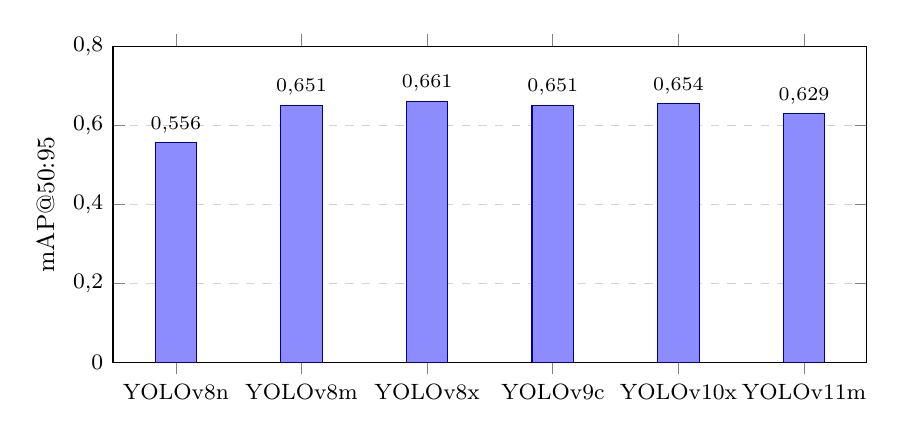
\begin{tikzpicture}
\begin{axis}[
  ybar, width=0.92\linewidth, height=5.6cm,
  symbolic x coords={YOLOv8n,YOLOv8m,YOLOv8x,YOLOv9c,YOLOv10x,YOLOv11m},
  xtick=data, ymin=0, ymax=0.8, bar width=15pt, enlarge x limits=0.10,
  ylabel={mAP@50:95},
  tick label style={font=\footnotesize}, label style={font=\small},
  nodes near coords, nodes near coords align={vertical},
  every node near coord/.append style={font=\scriptsize},
  /pgf/number format/.cd, fixed, precision=3, use comma,
  ymajorgrids=true, grid style={dashed,gray!35}]
\addplot[fill=blue!45, draw=blue!60!black] coordinates {(YOLOv8n,0.556) (YOLOv8m,0.651) (YOLOv8x,0.661) (YOLOv9c,0.651) (YOLOv10x,0.654) (YOLOv11m,0.629)};
\end{axis}
\end{tikzpicture}
\caption{Vrijednosti mAP@50:95 odabranih modela (rekonstrukcija objavljenih vrijednosti iz tabela 6--9 rada \cite{ramos}; nije eksperimentalni rezultat tima).}
\label{fig:dino-map}
\end{figure}

Najveći prijavljeni mAP@50:95 među analiziranim konfiguracijama dostiže YOLOv8x: 0,661. Blizu je YOLOv10x (0,654), ali uz sporije treniranje i nešto veću latenciju. Istovremeno, YOLOv8m (0,651) postiže skoro jednak kvalitet uz 3,4\,ms inferencije naspram 6,9\,ms kod YOLOv8x, što ga čini praktično interesantnim. YOLOv9c ima visok precision (0,872), ali kvalitativni testovi bilježe pogrešne detekcije dima. YOLOv11m bolji je od većih YOLOv11 varijanti, što potvrđuje da veličina mreže sama po sebi nije garancija napretka \cite{ramos}.

Važan detalj je neravnomjeran kvalitet po klasama: kod YOLOv8x mAP@50:95 iznosi 0,732 za dim, ali samo 0,589 za vatru. Iz toga slijedi da zbirna mAP metrika može prikriti slabiju detekciju pojedine klase. Na vizuelnim primjerima autori također navode da neki YOLOv10 i YOLOv11 modeli izbjegavaju lažne detekcije bolje od YOLOv8, dok svi modeli imaju poteškoće s jedva vidljivim dimom noću \cite{ramos}.

\subsubsection{Prednosti i nedostaci}
\textbf{Prednosti rada:}
\begin{enumerate}
  \item Jednaki osnovni uslovi treniranja olakšavaju poređenje arhitektura.
  \item Analizirani su i laki i veliki modeli, pa rezultati imaju značaj za različite hardverske budžete.
  \item Kombinacija statističkih metrika i pregledanih vizuelnih predikcija otkriva probleme koje jedna agregatna vrijednost mAP ne može pokazati.
  \item Navođenje latencije je važno zbog mogućih sistema ranog upozoravanja.
\end{enumerate}

\textbf{Ograničenja.} Autori sami navode oslanjanje na jedan skup podataka, koji ne predstavlja nužno sve vrste terena i vremenskih uslova, te izostavljanje alternativnih porodica detektora. Dodatno, naša procjena je da bi poređenje bilo uvjerljivije uz testiranje na potpuno nezavisnom skupu slika, ponavljanja s različitim nasumičnim sjemenima i detaljniju analizu lažnih alarma. Rezultati brzine zavise od korištenog hardvera. Bez zasebnog terenskog testa ne može se tvrditi da model radi jednako dobro na kamerama u Bosni i Hercegovini ili na jeftinim uređajima \cite{ramos}.

\subsubsection{Povezanost sa skupom D-Fire i smjernice}
Za projekat je odabran Smoke-Fire-Detection-YOLO (Kaggle). Autori originalnog skupa D-Fire izričito navode ovaj Kaggle link kao verziju spremnu za korištenje \cite{dfire,kaggle}. To nije isti skup kao Roboflow Fire and Smoke iz analiziranog rada. D-Fire ima 21.527 slika, od kojih su 1.164 samo s vatrom, 5.867 samo s dimom, 4.658 s obje klase i 9.838 bez njih; objavljeno je 14.692 okvira vatre i 11.865 okvira dima (ukupno 26.557), u YOLO formatu s normaliziranim koordinatama \cite{dfire}. Autori D-Fire skupa preporučuju citiranje publikacije de Venâncio i saradnika \cite{venancio}. Provjera tačnog rasporeda datoteka i indeksa klasa u preuzetoj Kaggle kopiji obavezna je prije treniranja.

\begin{table}[H]
\centering
\small
\begin{tabularx}{\linewidth}{@{}>{\raggedright\arraybackslash}p{3.8cm}>{\raggedright\arraybackslash}X>{\raggedright\arraybackslash}X@{}}
  \toprule
  \textbf{Osobina} & \textbf{Rad Ramos i sar.} & \textbf{Naš projekat -- D-Fire}\\
  \midrule
  Izvor & Roboflow: Fire and Smoke & Originalni D-Fire; Kaggle distribucija\\
  Broj slika & 9.796 & 21.527\\
  Klase & Vatra, dim & Vatra, dim\\
  Broj anotiranih objekata & 29.375 & 26.557\\
  Slike bez objekata & Nije precizirano u analizi & 9.838\\
  Anotacije & Okviri za detekciju & YOLO format (okviri)\\
  \bottomrule
\end{tabularx}
\caption{Relevantne razlike između skupa iz rada i projektne verzije skupa D-Fire \cite{ramos,dfire}.}
\label{tab:dino-razlike}
\end{table}

Velik broj negativnih slika (bez vatre i dima) u D-Fire skupu koristan je za ispitivanje lažnih alarma, ali zahtijeva pažljivo testiranje. Različita porijekla slika, broj anotacija i mogući odnos klasa znače da rezultati iz rada nisu direktno prenosivi na D-Fire; njihova vrijednost je metodološka, jer daju polazne hipoteze o izboru modela, mjera i kompromisa.

\paragraph{Smjernice za naredne laboratorijske vježbe.}
\begin{enumerate}
  \item \textbf{Priprema skupa:} učitati preuzeti D-Fire, pregledati \texttt{data.yaml}, oznake i odnos slika bez objekata; provjeriti duplikate i potencijalno preklapanje kadrova iz istog videa između skupova.
  \item \textbf{Reproducibilna podjela:} koristiti isporučeni train/validation/test raspored ako postoji i dokumentovati ga; u suprotnom napraviti fiksnu podjelu uz razdvajanje povezanih video-sekvenci.
  \item \textbf{Početni modeli:} trenirati YOLOv8n ili YOLOv8s kao računarski jeftin početni model, a YOLOv8m kao kandidata za bolju tačnost. Kao kontrolno poređenje testirati YOLOv10s ili YOLO11s, pri jednakim ulaznim dimenzijama i uslovima.
  \item \textbf{Evaluacija:} mjeriti mAP@50, mAP@50:95, precision i recall zasebno za vatru i dim, broj lažnih alarma na negativnim slikama, matricu konfuzije te latenciju na stvarnom hardveru.
  \item \textbf{Analiza grešaka:} izdvojiti primjere slabe vidljivosti, noćnih scena, oblaka i magle, sitnih plamenova i dima u daljini. Varijante augmentacije i prag pouzdanosti vrednovati isključivo na validacijskom skupu.
\end{enumerate}
Navedene smjernice su prijedlog našeg pristupa, a ne eksperimenti izvedeni u ovom LV2 niti rezultati koje su autori Ramos i saradnici prijavili.

\paragraph{Zaključak.} Rad pruža korisnu komparativnu osnovu za detekciju požara i dima: u datim eksperimentalnim uslovima YOLOv8 nudi najbolji ukupni odnos tačnosti i efikasnosti, a YOLOv10 je bliska alternativa koja u pojedinim vizuelnim scenarijima proizvodi manje lažnih detekcija. Za naš projekat sa skupom D-Fire razumno je započeti lakšim YOLOv8 modelom, zatim testirati srednju varijantu i jednu drugu arhitekturu, uz poseban naglasak na propuštene požare i lažne alarme. Konačan izbor ne može se napraviti bez treninga i nezavisnog testiranja na stvarno odabranom skupu podataka.

% =====================================================================
%  DIO 5 -- Haris Macić: Li i sar. (2025), GSF-YOLOv8
%
%  ISPRAVLJENO: bibliografski podaci (autori C. Li, D. Wu, X. Zhang,
%  P. Wu; IEEE Access, sv. 13, str. 66051--66064, 2025.) usklađeni su
%  s IEEE Xplore (https://ieeexplore.ieee.org/document/10964263/).
%  Izvorni izvještaj je navodio "X. Li, Y. Wang, H. Zhang", sv. 12, 2024.
% =====================================================================
\clearpage
\subsection{\texorpdfstring{\AutorE}{Haris Macić} --- GSF-YOLOv8: Gather-Distribute mehanizam i SimAM pažnja}

\paperbox{\AutorE}
  {C.\ Li, D.\ Wu, X.\ Zhang i P.\ Wu, „GSF-YOLOv8: A Novel Approach for Fire Detection Using Gather-Distribute Mechanism and SimAM Attention“ \cite{ligsf}}
  {\emph{IEEE Access}, sv.\ 13, str.\ 66051--66064, 2025.\ DOI: 10.1109/ACCESS.2025.3560393}
  {D-Fire (treniranje, ablacione studije i poređenje s drugim modelima)}
  {Novi model (modifikacija YOLOv8s) s eksperimentalnom evaluacijom}

\subsubsection{Sažetak}
Rad predlaže GSF-YOLOv8, modifikaciju modela YOLOv8s \cite{jocher} za detekciju vatre i dima na slikama sa nadzornih kamera. Motivacija je što tradicionalni detektori zasnovani na fizičko-hemijskim senzorima (toplota, CO$_2$) kasne, jer produkti sagorijevanja moraju stići do samog senzora, pa su na otvorenim prostorima gotovo neupotrebljivi. Sistemi računarskog vida to rješavaju obradom slike u realnom vremenu.

Standardni YOLO detektori optimizovani su za čvrste objekte stabilnih ivica (vozila, pješaci), pa pri detekciji požara imaju dva problema:
\begin{enumerate}
  \item \textbf{Degradacija prostornih informacija u piramidi karakteristika.} Standardne strukture FPN i PAN oslanjaju se na uzastopna spajanja susjednih nivoa odozgo prema dolje i odozdo prema gore; pri višestrukim konvolucijama i pooling operacijama fine prostorne informacije o malim žarištima plamena nepovratno se gube.
  \item \textbf{Neadekvatno modeliranje amorfnog dima.} Klasične pažnje (SE, CBAM) modeluju kanalske ili prostorne težine nezavisno, što nije dovoljno za praćenje poluprozirnih i difuznih oblaka dima bez definisanih kontura.
\end{enumerate}
Cilj autora je arhitektura koja smanjuje broj parametara i računarsku složenost osnovnog YOLOv8s modela, a istovremeno povećava osjetljivost na dim i male objekte plamena. Na skupu D-Fire model postiže mAP@0.5 od 80,65\% uz brzinu od 118 FPS \cite{ligsf}.

\subsubsection{Korištene metode}
\paragraph{Skup podataka.} Korišten je D-Fire (GAIA Solutions on Demand) \cite{dfire}: preko 20.000 anotiranih instanci u YOLO formatu s klasama \emph{fire} i \emph{smoke}, podijeljenih u četiri podgrupe: samo vatra (urbana i ruralna okruženja), samo dim (rano tinjanje, plamen još nije vidljiv ili je zaklonjen), vatra i dim (razvijeni požar) te neutralne slike bez požara koje sadrže vizuelno slične pojave (niski oblaci, gusta magla, prašina, industrijske emisije). Ključni izazovi su rani plamen koji zauzima svega nekoliko piksela te dim s amorfnim granicama i promjenljivom prozirnošću.

\paragraph{Predložena arhitektura.} Autori uvode tri modifikacije baznog YOLOv8 modela (Slika~\ref{fig:gsf}).
\begin{itemize}
  \item \textbf{Gather-Distribute (GD) mehanizam u vratu mreže.} Umjesto kaskadnog prosljeđivanja informacija kroz PANet, u fazi \emph{gather} karakteristike sa različitih skala okosnice se sakupljaju, poravnavaju na zajedničku dimenziju i agregiraju u globalni modul fuzije. U fazi \emph{distribute} tako fuzionisana reprezentacija se raspodjeljuje granama detektora niske, srednje i visoke rezolucije. Time se izbjegava gubitak informacija karakterističan za tradicionalne piramide, a glava za male objekte dobija direktan pristup globalnom kontekstu scene.
  \item \textbf{SimAM (\emph{Simple Parameter-Free Attention Module}).} Modul pojačava razlikovanje dima od magle i oblaka bez dodavanja novih parametara. Za razliku od standardnih 1D/2D pažnji, SimAM računa 3D raspodjelu pažnje optimizacijom energetske funkcije svakog neurona,
  \begin{equation}
    e_t(w_t, b_t, y, x_i) = \frac{1}{M-1}\sum_{i=1}^{M-1}\bigl(-1-(w_t x_i + b_t)\bigr)^2 + \bigl(1-(w_t t + b_t)\bigr)^2 + \lambda w_t^2,
  \end{equation}
  gdje je $t$ ciljni neuron unutar kanala, a $x_i$ su ostali neuroni. Što je energija $e_t$ niža, neuron se više razlikuje od okoline (veća vizuelna važnost) i dobija veću težinu.
  \item \textbf{Focal-DIoU funkcija gubitka za granične okvire.} Umjesto standardnog CIoU gubitka koristi se kombinacija Distance-IoU gubitka s dinamičkim fokusiranjem na teške primjere malih žarišta,
  \begin{equation}
    L_{\text{Focal-DIoU}} = \mathrm{IoU}^{\gamma}\cdot L_{\mathrm{DIoU}}, \qquad L_{\mathrm{DIoU}} = 1 - \mathrm{IoU} + \frac{\rho^{2}(b, b^{gt})}{c^{2}}.
  \end{equation}
  Faktor $\mathrm{IoU}^{\gamma}$ usmjerava učenje na preklapanja s malim ciljevima i ubrzava konvergenciju graničnih okvira plamena.
\end{itemize}

\begin{figure}[H]
\centering
\begin{tikzpicture}[node distance=0.75cm,
  st/.style={draw=black!70, rounded corners=2pt, fill=blue!6, text width=2.4cm, inner sep=4pt, align=center, minimum height=1.4cm, font=\footnotesize},
  arr/.style={-{Stealth[length=2mm]}, thick, black!70}]
  \node[st] (n1) {\textbf{Ulazna slika}\\ D-Fire, $640\times 640$};
  \node[st, right=of n1] (n2) {\textbf{Backbone (C2f)}\\ + SimAM (3D pažnja)};
  \node[st, right=of n2] (n3) {\textbf{Gather-Distribute}\\ (GD) fuzija};
  \node[st, right=of n3] (n4) {\textbf{Detekcijska glava}\\ (Focal-DIoU)};
  \draw[arr] (n1) -- (n2);
  \draw[arr] (n2) -- (n3);
  \draw[arr] (n3) -- node[above, font=\scriptsize]{P3, P4, P5} (n4);
\end{tikzpicture}
\caption{Strukturni dijagram toka podataka u GSF-YOLOv8 arhitekturi.}
\label{fig:gsf}
\end{figure}

\paragraph{Eksperimentalna postavka.} Eksperimenti su izvedeni na grafičkoj kartici NVIDIA RTX 3090 u PyTorch okruženju, uz ulaz $640\times 640$ piksela, 300 epoha i SGD optimizator.

\subsubsection{Ostvareni rezultati}
GSF-YOLOv8 ostvaruje najbolji mAP@0.5 (80,65\%) među poređenim modelima, što je poboljšanje od 1,75 procentnih poena u odnosu na teži YOLOv8s baseline. Broj parametara smanjen je sa 11,13\,M na 6,04\,M (oko 45,7\%), a računska složenost prepolovljena (sa 28,4 na 14,2 GFLOPs). Brzina izvođenja je 118 FPS \cite{ligsf}. Poređenje modela dato je u Tabeli~\ref{tab:gsf-poredjenje}, a doprinos pojedinih modula u Tabeli~\ref{tab:gsf-ablacija}.

\begin{table}[H]
\centering
\small
\setlength{\tabcolsep}{4pt}
\begin{tabular}{@{}lccccc@{}}
  \toprule
  \textbf{Model detektora} & \textbf{Param. (M)} & \textbf{GFLOPs} & \textbf{P (\%)} & \textbf{R (\%)} & \textbf{mAP@0.5 (\%)}\\
  \midrule
  YOLOv5s & 7,02 & 15,8 & 76,4 & 71,2 & 74,8\\
  YOLOv7-tiny & 6,20 & 13,7 & 77,8 & 73,1 & 76,5\\
  YOLOv8n & 3,15 & 8,1 & 74,2 & 69,8 & 72,5\\
  YOLOv8s (baseline) & 11,13 & 28,4 & 80,1 & 76,9 & 78,9\\
  \textbf{GSF-YOLOv8 (predloženi)} & \textbf{6,04} & \textbf{14,2} & \textbf{83,4} & \textbf{78,6} & \textbf{80,65}\\
  \bottomrule
\end{tabular}
\caption{Poređenje performansi različitih modela na skupu D-Fire.}
\label{tab:gsf-poredjenje}
\end{table}

\begin{table}[H]
\centering
\small
\begin{tabular}{@{}lcccc@{}}
  \toprule
  \textbf{Konfiguracija modela} & \textbf{Parametri (M)} & \textbf{Precision (\%)} & \textbf{Recall (\%)} & \textbf{mAP@0.5 (\%)}\\
  \midrule
  YOLOv8s baseline & 11,13 & 80,1 & 76,9 & 78,90\\
  + Low-GD mehanizam & 6,04 & 81,8 & 77,4 & 79,82\\
  + SimAM pažnja & 6,04 & 82,7 & 78,1 & 80,31\\
  + Focal-DIoU (kompletni GSF) & 6,04 & 83,4 & 78,6 & 80,65\\
  \bottomrule
\end{tabular}
\caption{Doprinos pojedinačnih modula prema ablacionoj studiji na skupu D-Fire.}
\label{tab:gsf-ablacija}
\end{table}
Ablaciona analiza pokazuje da najveći skok u kompresiji modela donosi zamjena vrata mreže Low-GD mehanizmom, dok SimAM pažnja i Focal-DIoU stabilizuju regresiju malih meta bez uticaja na veličinu težina.

\subsubsection{Prednosti i nedostaci}
\textbf{Prednosti:}
\begin{itemize}
  \item \textbf{Visoka računska efikasnost:} prepolovljen broj GFLOPs i manji broj parametara čine model pogodnim za implementaciju na rubnim uređajima (Edge AI), poput NVIDIA Jetson platformi, uz brzinu od 118 FPS.
  \item \textbf{Dobra selekcija pažnje:} SimAM uspješno filtrira pozadinsku buku (oblake i maglu) bez trošenja dodatne memorije, što je važno za neutralne slike u skupu D-Fire.
  \item Svaka od tri modifikacije ima mjerljiv doprinos u ablacionoj studiji.
\end{itemize}

\textbf{Nedostaci i ograničenja:}
\begin{itemize}
  \item \textbf{Složenost optimizacije za hardver:} iako model ima manje GFLOPs-a, Gather-Distribute struktura ima nelinearnije rute kretanja podataka od jednostavnog FPN-a, što može otežati INT8 TensorRT optimizaciju bez gubitka preciznosti.
  \item \textbf{Nedostatak vremenske komponente:} model evaluira svaku sliku nezavisno. U stvarnom video nadzoru statična detekcija dima i dalje je podložnija lažnim alarmima u poređenju sa sistemima koji prate optički tok ili vremensku ekspanziju.
  \item \textbf{Jedan skup podataka:} evaluacija je rađena na skupu D-Fire, pa je generalizacija na druge scenarije nepoznata, a brzinu (118 FPS) treba ponovo izmjeriti na hardveru koji ćemo koristiti.
\end{itemize}

\subsubsection{Povezanost sa skupom D-Fire i smjernice}
Rad direktno koristi D-Fire za treniranje, ablacione studije i komparativnu validaciju sa stanjem tehnike, pa je njegov rezultat (mAP@0.5 = 80,65\%) neposredno uporediv s onim što možemo očekivati na istom skupu. Rad pokazuje da standardni YOLOv8 ima prostora za znatnu optimizaciju kada se primjenjuje na specifične zadatke poput detekcije vatre i dima. Za naš praktični rad nad skupom D-Fire korisno je preuzeti tri ideje:
\begin{enumerate}
  \item korištenje laganih modula pažnje (poput SimAM-a) u ranoj fazi ekstrakcije obilježja;
  \item poseban tretman neutralnih pozadinskih slika iz skupa D-Fire tokom treniranja radi suzbijanja lažnih alarma;
  \item primjena naprednih funkcija gubitka (Focal-DIoU ili Wise-IoU) za bolje pozicioniranje graničnih okvira na malim žarištima.
\end{enumerate}

% =====================================================================
%  DIO 6 -- Adnan Šemić: Li i sar. (2025), YOLOGX
%  Tabela rezultata provjerena prema Tabeli 4 izvornog rada (Frontiers).
% =====================================================================
\clearpage
\subsection{\texorpdfstring{\AutorF}{Adnan Šemić} --- YOLOGX: unaprijeđeni YOLOv8 za detekciju šumskih požara}

\paperbox{\AutorF}
  {C.\ Li, Y.\ Du, X.\ Zhang i P.\ Wu, „YOLOGX: an improved forest fire detection algorithm based on YOLOv8“ \cite{liyologx}}
  {\emph{Frontiers in Environmental Science}, sv.\ 12, čl.\ 1486212, 2025.\ DOI: 10.3389/fenvs.2024.1486212}
  {D-Fire (oko 21.500 slika; podjela 80:20)}
  {Novi model (modifikacija YOLOv8) s eksperimentalnom evaluacijom}

\subsubsection{Sažetak}
Rad predstavlja unaprijeđeni algoritam za automatsko prepoznavanje šumskih požara na slikama. Cilj istraživanja bio je poboljšati preciznost detekcije vatre i dima, posebno u složenim uslovima kao što su promjenljivo osvjetljenje, različite pozadine i prisustvo manjih objekata.

Autori su razvili model YOLOGX na osnovu postojeće arhitekture YOLOv8, uvodeći izmjene u načinu izdvajanja i povezivanja vizuelnih karakteristika, detekcijsku glavu i funkciju gubitka. Model je testiran na skupu D-Fire, koji sadrži slike vatre, dima, njihove istovremene pojave te slike bez vatre i dima. Rezultati pokazuju da predloženi model postiže mAP@0.5 od 80,92\% i brzinu obrade od 115 slika u sekundi. Istraživanje pokazuje da se izmjenama standardnog YOLOv8 modela može poboljšati detekcija požara, uz zadržavanje brzine pogodne za primjenu u sistemima za nadzor u realnom vremenu \cite{liyologx}.

\subsubsection{Korištene metode}
Osnovu rješenja čini YOLOv8, metoda dubokog učenja za detekciju objekata na slikama. Za razliku od klasifikacije, koja određuje kojoj kategoriji slika pripada, detekcija objekata prepoznaje prisutne kategorije i određuje njihove lokacije pomoću graničnih okvira. U ovom radu model se koristi za prepoznavanje i lokalizaciju vatre i dima.

YOLOGX uvodi tri glavne izmjene:
\begin{itemize}
  \item \textbf{Gather-Distribute (GD) mehanizam:} povezuje informacije iz različitih nivoa mreže. Na taj način model kombinuje lokalne detalje i širi kontekst slike, što pomaže pri prepoznavanju objekata različitih veličina.
  \item \textbf{SE-ResNeXt detekcijska glava:} koristi grupne konvolucije i mehanizam pažnje nad kanalima kako bi efikasnije izdvajala važne karakteristike slike, čime se nastoji poboljšati prepoznavanje relevantnih karakteristika vatre i dima.
  \item \textbf{Focal-SIoU funkcija gubitka:} koristi se tokom treniranja radi poboljšanja predviđanja graničnih okvira. U obzir uzima preklapanje, udaljenost, oblik i ugaone odnose između predviđenih i stvarnih okvira, uz dodatno prilagođavanje doprinosa različitih primjera treniranju.
\end{itemize}

Model je treniran i testiran na skupu D-Fire, koji obuhvata oko 21.500 slika. Autori su koristili podjelu podataka za treniranje i testiranje u omjeru približno 80:20, uz tehnike proširenja podataka kao što su izrezivanje i okretanje slika. Uspješnost su procjenjivali pomoću preciznosti, odziva, mAP-a i brzine obrade izražene u broju slika u sekundi (FPS).

\subsubsection{Ostvareni rezultati}
Eksperimentalni rezultati pokazuju da YOLOGX ostvaruje bolje rezultate od osnovnog YOLOv8 modela prema pojedinim važnim pokazateljima. Najveće poboljšanje ostvareno je u odzivu (\emph{recall}) i mAP@0.5, što ukazuje na bolju sposobnost pronalaska relevantnih objekata na slikama (Tabela~\ref{tab:yologx}).

\begin{table}[H]
\centering
\small
\begin{tabular}{@{}lcc@{}}
  \toprule
  \textbf{Pokazatelj} & \textbf{YOLOv8} & \textbf{YOLOGX}\\
  \midrule
  Preciznost (\%) & 78,80 & 77,20\\
  Odziv (\%) & 72,50 & 75,70\\
  mAP@0.5 (\%) & 79,46 & 80,92\\
  mAP@0.5--0.95 (\%) & 46,61 & 46,44\\
  Brzina (FPS) & 197 & 115\\
  Broj parametara & 3,0\,M & 6,2\,M\\
  \bottomrule
\end{tabular}
\caption{Poređenje osnovnog YOLOv8 i YOLOGX modela na skupu D-Fire (prema \cite{liyologx}).}
\label{tab:yologx}
\end{table}

Vrijednost mAP@0.5 povećana je sa 79,46\% na 80,92\%, dok je odziv povećan sa 72,50\% na 75,70\%. Veći odziv znači da model uspješnije pronalazi objekte koji zaista postoje na slikama. Međutim, preciznost je smanjena sa 78,80\% na 77,20\%, što ukazuje na određeni kompromis između pronalaženja većeg broja objekata i izbjegavanja lažnih detekcija. Brzina obrade smanjena je sa 197 na 115 FPS, a broj parametara povećan je sa 3,0 miliona na 6,2 miliona. Ipak, 115 FPS i dalje predstavlja visoku brzinu obrade za primjene u realnom vremenu. Rezultati zato pokazuju da YOLOGX poboljšava određene aspekte detekcije, ali uz povećane računarske zahtjeve.

\subsubsection{Prednosti i nedostaci}
\textbf{Prednosti:}
\begin{itemize}
  \item YOLOGX postiže veći mAP@0.5 i odziv u odnosu na osnovni YOLOv8.
  \item GD mehanizam omogućava povezivanje informacija različitih nivoa, što je korisno za prepoznavanje vatre i dima različitih veličina.
  \item Dodatne izmjene poboljšavaju izdvajanje karakteristika i preciznost lokalizacije objekata.
  \item Brzina od 115 FPS pokazuje da model ima potencijal za primjenu u sistemima koji zahtijevaju brzu analizu slike.
\end{itemize}

\textbf{Nedostaci:}
\begin{itemize}
  \item Unaprijeđeni model ima manju brzinu obrade i veći broj parametara od osnovnog YOLOv8, pa može zahtijevati snažniji hardver.
  \item Preciznost je nešto niža, a mAP@0.5--0.95 blago je smanjen sa 46,61\% na 46,44\%.
  \item Rezultati dobijeni na jednom skupu podataka ne garantuju jednaku uspješnost u svim stvarnim uslovima. Promjene osvjetljenja, složene pozadine, magla i slične pojave mogu otežati razlikovanje dima i vatre od drugih vizuelno sličnih objekata.
\end{itemize}

\subsubsection{Povezanost sa skupom D-Fire i zaključak}
Rad je evaluiran na skupu D-Fire, pa su njegovi rezultati neposredno relevantni za naš projekat: osnovni YOLOv8 na tom skupu postiže mAP@0.5 od 79,46\%, što je dobar orijentir za naš baseline, a YOLOGX pokazuje koliko se može dobiti dodatnim izmjenama (GD mehanizam, SE-ResNeXt glava, Focal-SIoU gubitak). Pritom treba imati na umu kompromis između tačnosti, brzine i broja parametara.

Zaključno, YOLOGX predstavlja unapređenje YOLOv8 pristupa za detekciju šumskih požara. Model ostvaruje bolje rezultate prema mAP@0.5 i odzivu, ali uz smanjenje brzine i povećanje broja parametara. Zbog toga je pri izboru modela potrebno razmotriti odnos između preciznosti, brzine i dostupnih računarskih resursa.